\chapter{Structured Characters}
This chapter presents a concept to embed structured data in an atomic character. It enables the use of structured data, like \code{EObjects} on the character input stream for the Lexer. In combination with typing rules, serialized notation model elements resolve to sentential forms of a word. The general idea is to use private characters as keys for a map. These special characters, which identify an object are called \emph{ID Characters} in the following.

\section{General Requirements}
The task of an ID Character is to uniquely identify an object in a serializable context. 
The ideal characteristics are:
\begin{itemize}
	\item bindable and existence dependent on another character or standalone.
	\item unlimited number of unique identifiers.
	\item atomic. The integrity should be preserved and not be unbreakable.
	\item standardized. There should be a long term guarantee that their are available for use.
	\item ubiquitous available. They should be available on every platform.
	\item abstract characters. They should be fast distinguishable from non ID character.
	\item private. They should not causes any conflicts or be missinterpretable in any way.
\end{itemize}

\subsection{Unicode Private-Use Characters}
A possible solution offers Unicode \cite{Unicode}. Unicode is a universal character encoding standard for consistent encoding and exchange of text data. It is the default encoding of HTML and XML and is implemented in all modern operating systems. It specifies a numeric value (code point) and name for each character. Unicode was developed in conjunction with the Universal Character Set and can be represented by widely available encodings like UTF-8. The Unicode Standard defines private-use characters, which interpretation is not specified and is determined by a private agreement among cooperative users. For example Apple uses a private character to present it's apple logo. A application specific changed interpretation of for example the character representing the apple logo is valid, as it specifies its intended behavior according to a private agreement.\\
The private use characters are intended for software developers. They can be compared to the ideal characteristics:
\begin{itemize}
	\item they are stand alone characters and are not bindable per se.
	\item The number of identifiers is limited to 137,468, in which 6,400 are in the private use area U+E000 to U+F8FF and 65,534 are in each supplementary private use Area-A and Area-B. 
	\item They are single characters and thus atomic. 
	\item Unicode is standardized and private-use characters are permanently designated for private use.
	\item Unicode, especially the UTF-8 encoding is wide spread and nearly ubiquitous available on modern personal computer platforms.
	\item There are three code-blocks for private-use characters. Three range check for a code point is in sufficient to determine its private-use.
	\item Private-use characters are, as the name states, explicitly designed for private use.
\end{itemize}
The restriction of a limited number of available identifiers could be solved by implementing a non-standard character encoding, probably a variable-with encoding.


%% Impl of ID Chars >>>>>>>>
\section{Use and implementation of ID-Characters}
 
The ID character can be to
\begin{itemize}
	\item add an ID to another token.
	\item use the ID to refer to an object.
\end{itemize}
In both cases, additional data must be preserved. Because the character stream used for serialization, the additional data should also be serialized in an adjacent file. Figure \ref{EMFLexer} sketches an EMF based Lexer extension. The adjacent file is named \code{EMF Document} on the right, whereas the token stream is read from the \code{Text Document} at the bottom. The wrapping Lexer is named \code{EMF Lexer} in figure \ref{EMFLexer}, whereas the wrapped Lexer is called \code{Original Lexer}.  

% ID giving
\paragraph{Adding an Identifier} To add an identifier to the following or previous token is useful in regard to enable stable references and enhance compare based updated approaches. This identifier providing use is \emph{not of interest for this thesis}. An associativity flag is required for right, none or left associativity.  Right associativity is easy to implement, because the wrapping Lexer can distinguish and filter the ID character, resolve the identifier and append it to the token value of the token returned by the wrapped Lexer. If left associativity may occur, this requires the wrapping Lexer to additionally cache one token of the wrapped Lexer and request another token from the wrapped Lexer. Aside easily distinguishable from the normal textual representation, ID characters clutter the output and should not be considered human readable without preprocessing. 
 
% ref EObject 
\paragraph{Referring character} \label{lexer:RefEObj} Using the ID character to refer to objects conceptually enables structured data on the character stream. This even exceeds the complexity of normal token values, which contain a sequence of characters in general. Restricting the referred objects to be serializable would be sufficient, but restricting the references to \code{EObject} eliminates impedance mismatch for an character to \code{EObject} mapping and also ensures a non binary XMI serialization. Figure \ref{EMFLexer} realizes this by a map from UTF8 character to a triple, $c \rightarrow (o,a,i)$, where $o$ is the referred object, $a$ is the associativity and $i$ is the extrinsic identifier. The associativity determines if it's a plain ID or as a reference character. \code{None} associative characters are EObject references. $o$ and $i$ can be a tree structures, because if $o$ contains other \code{EObject}s, multiple UUIDs adjacent to each \code{EObject} must be persisted in $i$. References between the serialized \code{EObject}s are by the use of UUIDs stable, but stability of references to textually described \code{EObject}s depend on the quality of the resource implementation and are problematic. \\
The workflow of an \code{EMF Lexer} is so far:
\begin{enumerate}
	\item Load the adjacent document and make the keys available.
	\item wait for a next token request.
	\item forwards this request to the \code{Original Lexer} and pass the regular characters on the input stream through to him.
	\item if the lexer produces a token, return it
	\item if the UTF8 private use character occurs, let the \code{EMF Lexer} handle it:
		\begin{itemize}
			\item resolve the triple and the according \code{EObject}
			\item save the UUID, either at the token by a value, or as a reference on the \code{EObject} or as an adapter attached to the \code{EObject} 
		\end{itemize} 
	\item Test if specialization \code{Typer Rules} exist, and if it does not assume the grammar explicitly defined this type and assign the classname of the \code{EObject} to the token name. Finally assign the resolved \code{EObject} to the tokens \code{value}.
\end{enumerate}

\paragraph{Referring Sentential Forms}
The assignment of the tokens name is  static in \ref{lexer:RefEObj} ,the previous solution. To leverage the approach of letting the lexical analyzer return \code{EObject}s, the token name can be determined by rules. These rules can be added to, and interpreted by the \code{EObject Typer}. The \code{Typer Rules} process the input \code{EObject} and assign the token name based on runtime analysis of the input. Sentential forms are serialized using the notation model. To enable the reference to sentential forms, an \code{EObject Typer} rule is necessary which assigns the token name properly. \\
The workflow of \ref{lexer:RefEObj} is extended by a \code{Typer Rule}, which performs:
\begin{enumerate}
	\item test the input \code{EObject} if it is an instance of \code{AlterableElement}. If it is not, the rule is not applied.
	\item test if the input is an instance of \code{NotationModel:List}. 
	If it is not a \code{List}:
	\begin{enumerate}
		\item resolve the grammar element by following the \code{notTerminal}, \code{sequence} or \code{terminal} reference. 
		\item for \code{Symbol}s, resolve their more generic referred \code{TerminalType} or \code{Rule}.
		\item determine their URI and assign it to the token name.
		\item assign the referred language element \code{EObject} to the tokens value.
		\item optionally validate if the language element structure comply to all constraints for the resolved grammar element.
	\end{enumerate}
	\item if the current \code{EObject} is a \code{List}, the \code{EMF Lexer} returns multiple tokens for a single character:
	\begin{itemize}
		\item remove the \code{AlterableElement} at the head of the list and resolve it like a stand alone element in the above steps.
		\item keep the smaller \code{List} on the input stream or redirect the next \kode{nextToken()} from the Lexer directly the current \code{Typer Rule}.  
	\end{itemize}
\end{enumerate}

The set of terminals is composed of: \\
$Terminals = Terminals_{OriginalLexer} \bigcup Terminals_{EMFObjects} \bigcup Terminals_{Sentential} \label{TotalTerminals}$

\begin{figure}
\centering
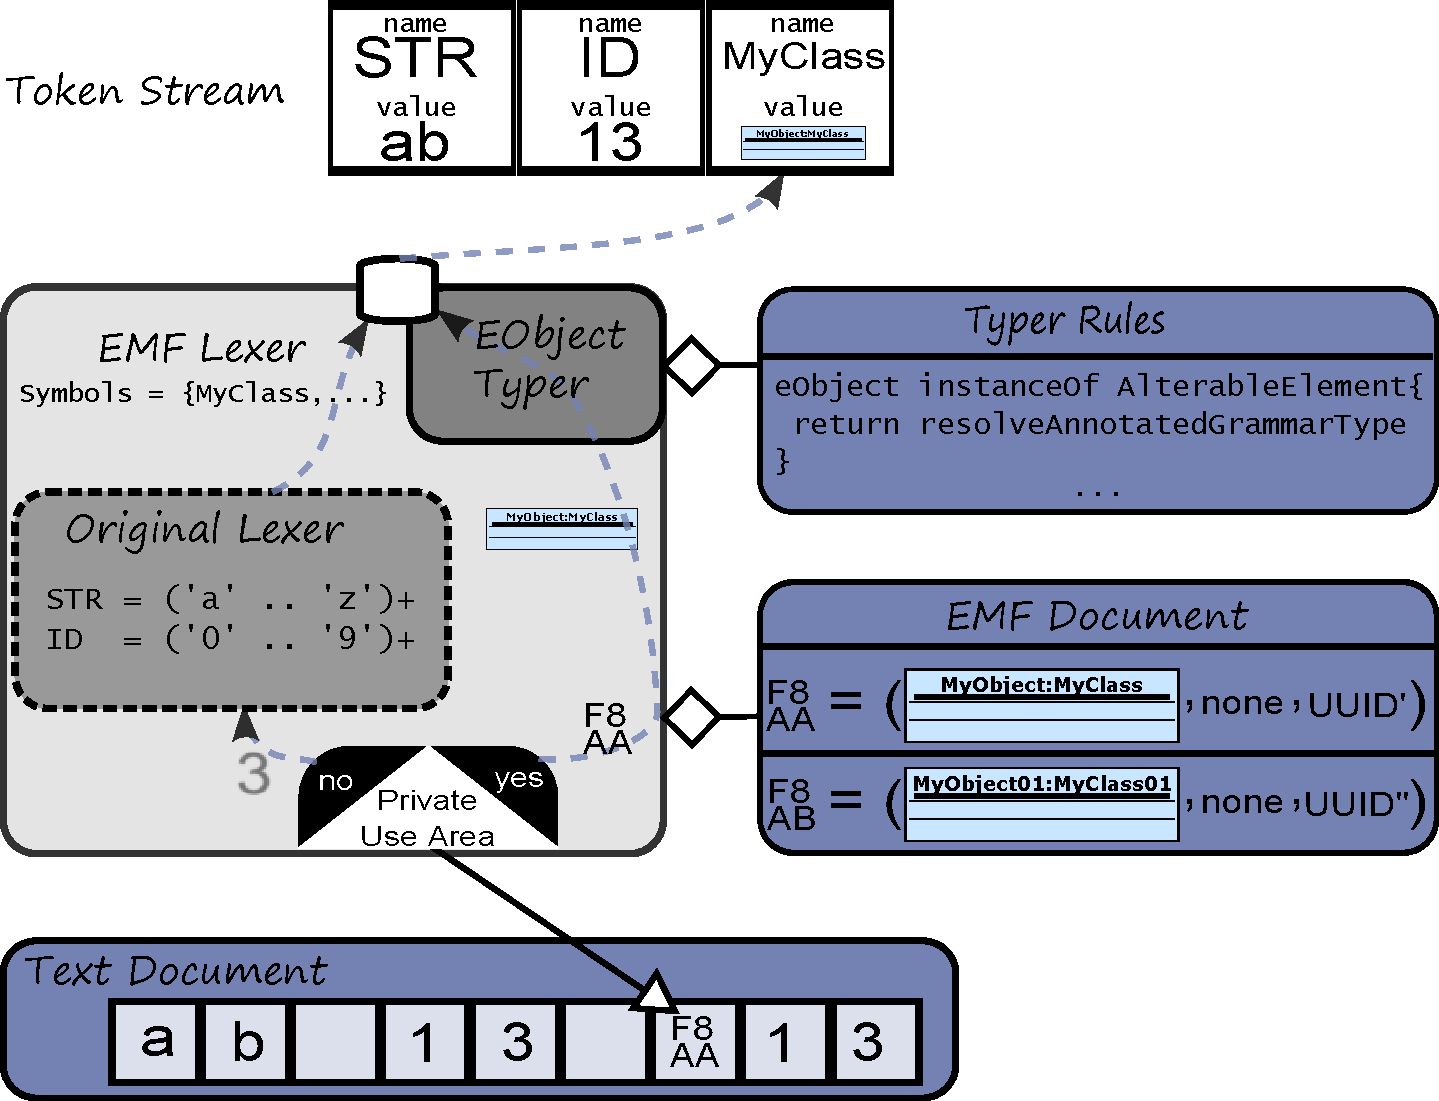
\includegraphics[scale=0.61]{gfx/ex/Lexer} 
\caption{EMF Lexer extension}
\label{EMFLexer}
\end{figure}
